\chapter{Evaluation}
\label{chap:eval}

This chapter evaluates the performance of \betrfs with
range-rename (\betrfsFour) and \betrfs with range-clone (\betrfsFive),
comparing them with widely used file systems and \betrfsThree.
\betrfsThree is the relative-path-indexed \betrfs that taxes other file system
operations for good namespace operations.
The evaluation includes both micro and macro benchmarks.

We seek to answer the following questions in the evaluation:
\begin{itemize}
\item How do non-namespace operations perform on \betrfsFour and \betrfsFive?
\item How do namespace operations perform on \betrfsFour and \betrfsFive?
\item Do applications perform well on \betrfsFour adn \betrfsFive?
\item Do \betrfsFour and \betrfsFive maintain good performance against file
    system aging?
\end{itemize}

\paragraph{Experimental Setup.}

All experimental results were collected on
a Dell Optiplex 790 with a 4-core 3.40 GHz Intel Core i7-2600 CPU,
4GB RAM,
and a 128 GiB partition (the rest of the disk is not used)
of a 500 GB, 7200 SATA disk with a 4096-byte block size
(Seagate Barracuda ST500DM002).
The system runs 64-bit Ubuntu server 14.04.6 on a USB stick to prevent
interference from the root file system.
\betrfsThree and \betrfsFour run on a modified Linux 3.11.10 kernel that
enlarges the size of the kernel stack,
while \betrfsFive and all other file systems run on Linux 4.9.142 kernel.
The evaluation uses ZFS 0.6.5.11 from \url{zfsonlinx.org} and
ext4, Btrfs, XFS and NILFS2 as parts of the Linux kernel.
Each experiment runs a minimum of 5 times and reports the average number.
Error bars indicate (95\%) confidence intervals over all runs.
Similarly, error $\pm$ terms show confidence intervals over all runs.
Unless noted, all benchmarks are cold-cache tests.

We run benchmarks on empty file systems and aged file systems.
We age the file system by emulating user behaviors.
First, we fill the file system with files and directories from the root file
system, roughly taking up 31 GiB space.
Then, we clone the git repository of the Linux kernel with the release tag
``v3.12'' (released on 2013/11/03) to the home directory in the file system.
Afterwards, we repeat the process of building the kernel and pulling the next
release of the repository
until we build the Linux kernel with the release tag ``v4.20''
(released on 2018/12/13).
This process takes several days to complete (about 5 days on ext4),
building the kernel 240 times
(though there are only 29 major releases, there are 7 to 9 release candidates
between two consecutive major releases)
and pulling 397,481 git commits.
The directory of the git repository takes up about 3.6 GiB space and
after building the kernel, it takes up about 15 GiB space.
Therefore, after the aging process, the whole file system takes up about 46 GiB
space, about 36\% of the partition size.
Unless otherwise noted, when benchmarking on aged file systems,
all operations are performed in the aged git repository.

\section{Microbenchmarks}
\label{sec:micro}

In this section we run file systems on microbenchmarks,
each measures the performance of one file system operations.
We divide file system operations into non-namespace operations
(Section~\ref{sec:micro:nnso})
and namespace operations (Section~\ref{sec:micro:nso}).

\subsection{Non-namespace operations}
\label{sec:micro:nnso}

\newcommand{\addSeqPlot}[1]{
    \addplot[
        discard if not={fs}{#1},
        fill=\pgfkeysvalueof{/fs-colors/#1},
        nodes near coords=\pgfkeysvalueof{/fs-names/#1},
    ]
    plot[
        error bars/.cd,
        y dir=both, y explicit,
    ]
    table[
        x=op,
        y=avg,
        y error plus expr=\thisrow{ci},
        y error minus expr=\thisrow{ci},
    ]
    {./data/seq_io.csv};
}

\newcommand{\addSeqPlotAged}[1]{
    \addplot[
        discard if not={fs}{#1},
        fill=\pgfkeysvalueof{/fs-colors/#1},
        nodes near coords=\pgfkeysvalueof{/fs-names/#1},
    ]
    plot[
        error bars/.cd,
        y dir=both, y explicit,
    ]
    table[
        x=op,
        y=avg,
        y error plus expr=\thisrow{ci},
        y error minus expr=\thisrow{ci},
    ]
    {./data/seq_io_aged.csv};
}

\begin{figure}[t]
    \begin{subfigure}{\textwidth}
        \centering
        \begin{tikzpicture}[yscale=0.95, xscale=0.95]
            \begin{axis}[
                    ybar,
                    ymin=0,
                    ymax=150,
                    ylabel={Bandwidth (MiB/sec)},
                    ymajorgrids=true,
                    symbolic x coords={seq.write,seq.read},
                    xtick={seq.write,seq.read},
                    xticklabels={write,read},
                    enlarge x limits=0.5,
                    visualization depends on=y \as \rawy,
                    xtick pos=right,
                    major tick length=0in,
                    xticklabel pos=right,
                    nodes near coords style={font=\small,anchor=east,rotate=90,xshift=-\pgfplotsunitylength*\rawy,},
                    height=.45\linewidth,
                    width=\linewidth,
                ]
                \addSeqPlot{ext4};
                \addSeqPlot{btrfs};
                \addSeqPlot{xfs};
                \addSeqPlot{zfs};
                \addSeqPlot{nilfs2};
                \addSeqPlot{betrfs3};
                \addSeqPlot{betrfs4};
                \addSeqPlot{betrfs5};
            \end{axis}
        \end{tikzpicture}
        \caption{\label{subfig:seq_io}Benchmarking on empty file systems.}
    \end{subfigure}
    \begin{subfigure}{\textwidth}
        \centering
        \begin{tikzpicture}[yscale=0.95, xscale=0.95]
            \begin{axis}[
                    ybar,
                    ymin=0,
                    ymax=150,
                    ylabel={Bandwidth (MiB/sec)},
                    ymajorgrids=true,
                    symbolic x coords={seq.write,seq.read},
                    xtick={seq.write,seq.read},
                    xticklabels={write,read},
                    enlarge x limits=0.5,
                    visualization depends on=y \as \rawy,
                    xtick pos=right,
                    major tick length=0in,
                    xticklabel pos=right,
                    nodes near coords style={font=\small,anchor=east,rotate=90,xshift=-\pgfplotsunitylength*\rawy,},
                    height=.45\linewidth,
                    width=\linewidth,
                ]
                \addSeqPlotAged{ext4};
                \addSeqPlotAged{btrfs};
                \addSeqPlotAged{xfs};
                \addSeqPlotAged{zfs};
                \addSeqPlotAged{nilfs2};
                \addSeqPlotAged{betrfs3};
                \addSeqPlotAged{betrfs4};
                \addSeqPlotAged{betrfs5};
            \end{axis}
        \end{tikzpicture}
        \caption{\label{subfig:seq_io_aged}Benchmarking on aged file systems.}
    \end{subfigure}
    \caption[Sequential-write and sequential-read benchmark]{\label{fig:seq_io}
        Bandwidth to sequentially read and write a 10 GiB file (higher is better).}
\end{figure}

\begin{table}[t]
    \begin{subtable}[b]{.5\textwidth}
    \centering
        \begin{tabular}{l|.@{${}\pm{}$}.}
        \hline
        File system & \multicolumn{2}{c}{random write (sec)} \\
        \hline
        \hline
        \input{./data/rand_io.csv}
        \hline
        \end{tabular}
        \caption{\label{subtab:rand_io}Benchmarking on empty file systems.}
    \end{subtable}
    \begin{subtable}[b]{.5\textwidth}
    \centering
        \begin{tabular}{l|.@{${}\pm{}$}.}
        \hline
        File system & \multicolumn{2}{c}{random write (sec)} \\
        \hline
        \hline
        \input{./data/rand_io_aged.csv}
        \hline
        \end{tabular}
        \caption{\label{subtab:rand_io_aged}Benchmarking on aged file systems.}
    \end{subtable}
    \caption[Random-write benchmark]{\label{tab:rand_io}
        Time to perform 256K (262,144) 4-Byte random writes one a 10GiB file (1 MiB total IO, lower is better).}
\end{table}

\begin{table}[t]
    \begin{subtable}{\textwidth}
        \centering
        \begin{tabular}{l|.@{${}\pm{}$}..@{${}\pm{}$}..@{${}\pm{}$}.}
        \hline
        File system & \multicolumn{2}{c}{grep (sec)} & \multicolumn{2}{c}{find (sec)} & \multicolumn{2}{c}{delete (sec)} \\
        \hline
        \hline
        \input{./data/dir_ops.csv}
        \hline
        \end{tabular}
        \caption{\label{subtab:dir_ops}Benchmarking on empty file systems.}
    \end{subtable}
    \begin{subtable}{\textwidth}
        \centering
        \begin{tabular}{l|.@{${}\pm{}$}..@{${}\pm{}$}..@{${}\pm{}$}.}
        \hline
        File system & \multicolumn{2}{c}{grep (sec)} & \multicolumn{2}{c}{find (sec)} & \multicolumn{2}{c}{delete (sec)} \\
        \hline
        \hline
        \input{./data/dir_ops_aged.csv}
        \hline
        \end{tabular}
        \caption{\label{subtab:dir_ops_aged}Benchmarking on aged file systems.}
    \end{subtable}
    \caption[Directory operation benchmark]{\label{tab:dir_ops}
        Time to perform recursive grep, find and delete of the Linux source directory (lower is better).}
\end{table}

\newcommand{\addTokubenchPlotAged}[1]
{
    \addplot[
        color=\pgfkeysvalueof{/fs-colors/#1},
        line width=0.75pt,
        mark=\pgfkeysvalueof{/fs-marks/#1},
    ]
    plot[
    ]
    table[
    ]
    {./data/toku_aged/#1.csv};
    \addlegendentry{\pgfkeysvalueof{/fs-names/#1}}
}

\begin{figure}[t]
    \begin{subfigure}{\textwidth}
        \centering
        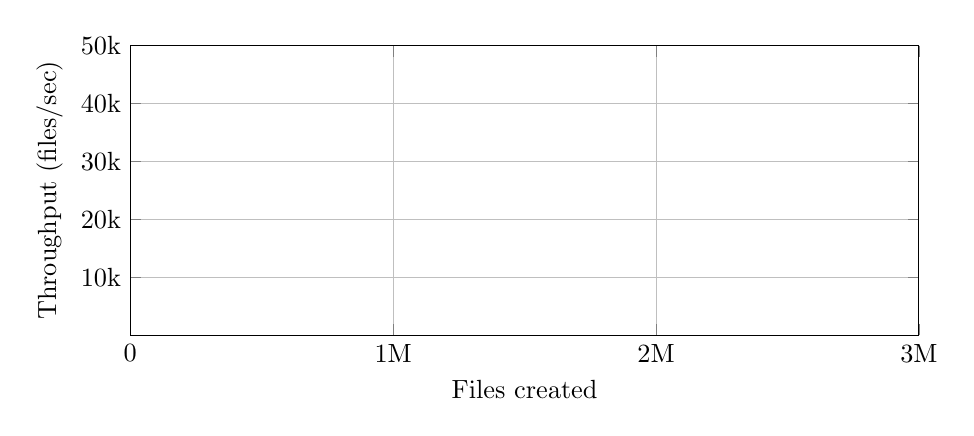
\begin{tikzpicture}[yscale=0.95, xscale=0.95]
            \begin{axis}[
                    xlabel={Files created},
                    ylabel={Throughput (files/sec)},
                    xmin=0,
                    xmax=3000000,
                    ymin=10,
                    ymax=50000,
                    mark repeat=10,
                    ytick={10000,20000,30000,40000,50000},
                    yticklabels={10k,20k,30k,40k,50k},
                    xtick={0,1000000,2000000,3000000},
                    xticklabels={0,1M,2M,3M},
                    grid=major,
                    scaled x ticks=false,
                    scaled y ticks=false,
                    legend columns=4,
                    legend cell align=left,
                    transpose legend,
                    height=.45\linewidth,
                    width=\linewidth,
                ]
                \addTokubenchPlot{ext4};
                \addTokubenchPlot{btrfs};
                \addTokubenchPlot{xfs};
                \addTokubenchPlot{zfs};
                \addTokubenchPlot{nilfs2};
                \addTokubenchPlot{betrfs3};
                \addTokubenchPlot{betrfs4};
                \addTokubenchPlot{betrfs5};
            \end{axis}
        \end{tikzpicture}
        \caption{\label{subfig:toku}Benchmarking on empty file systems.}
    \end{subfigure}
    \begin{subfigure}{\textwidth}
        \centering
        \begin{tikzpicture}[yscale=0.95, xscale=0.95]
            \begin{axis}[
                    xlabel={Files created},
                    ylabel={Throughput (files/sec)},
                    xmin=0,
                    xmax=3000000,
                    ymin=10,
                    ymax=50000,
                    mark repeat=10,
                    ytick={10000,20000,30000,40000,50000},
                    yticklabels={10k,20k,30k,40k,50k},
                    xtick={0,1000000,2000000,3000000},
                    xticklabels={0,1M,2M,3M},
                    grid=major,
                    scaled x ticks=false,
                    scaled y ticks=false,
                    legend columns=4,
                    legend cell align=left,
                    transpose legend,
                    height=.45\linewidth,
                    width=\linewidth,
                ]
                \addTokubenchPlotAged{ext4};
                \addTokubenchPlotAged{btrfs};
                \addTokubenchPlotAged{xfs};
                \addTokubenchPlotAged{zfs};
                \addTokubenchPlotAged{nilfs2};
                \addTokubenchPlotAged{betrfs3};
                \addTokubenchPlotAged{betrfs4};
                \addTokubenchPlotAged{betrfs5};
            \end{axis}
        \end{tikzpicture}
        \caption{\label{subfig:toku_aged}Benchmarking on aged file systems.}
    \end{subfigure}
    \caption[TokuBench benchmark]{\label{fig:toku}
        Cumulative file creation throughput during the Tokubench benchmark (higher is better).}
\end{figure}

\newcommand{\addFileRenamePlotAged}[1]
{
    \addplot[
        color=\pgfkeysvalueof{/fs-colors/#1},
        line width=0.75pt,
        mark=\pgfkeysvalueof{/fs-marks/#1},
    ]
    plot[
    ]
    table[
    ]
    {./data/file_rename_aged/#1.csv};
    \addlegendentry{\pgfkeysvalueof{/fs-names/#1}}
}

\begin{figure}[t]
    \begin{subfigure}{\textwidth}
        \centering
        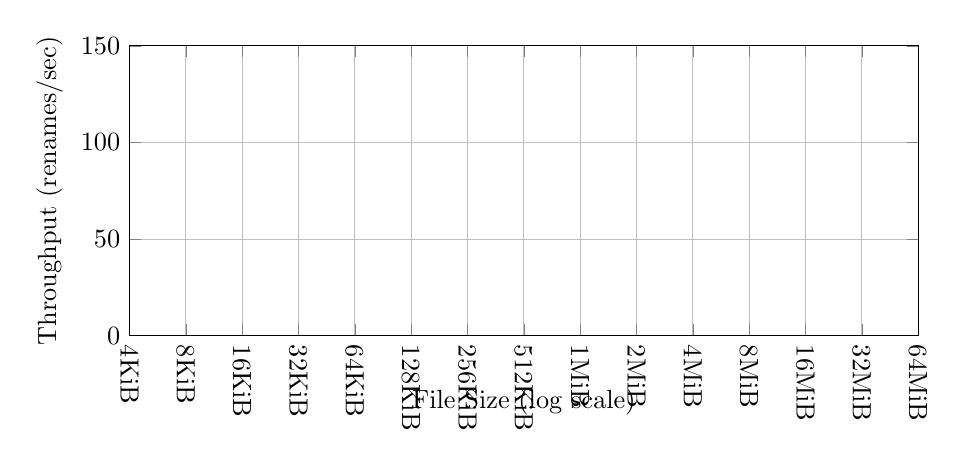
\begin{tikzpicture}[yscale=0.95, xscale=0.95]
            \begin{axis}[
                    xlabel={File Size (log scale)},
                    x label style={at={(axis description cs:0.5,-0.15)},anchor=north},
                    ylabel={Throughput (renames/sec)},
                    xmin=12,
                    xmax=26,
                    xtick={12,13,14,15,16,17,18,19,20,21,22,23,24,25,26},
                    xticklabels={4KiB,8KiB,16KiB,32KiB,64KiB,128KiB,256KiB,512KiB,1MiB,2MiB,4MiB,8MiB,16MiB,32MiB,64MiB},
                    xticklabel style={rotate=270, anchor=west},
                    ymin=0,
                    ymax=150,
                    grid=major,
                    scaled x ticks=false,
                    scaled y ticks=false,
                    legend columns=4,
                    legend cell align=left,
                    height=.45\linewidth,
                    width=\linewidth,
                ]
                \addFileRenamePlot{ext4};
                \addFileRenamePlot{btrfs};
                \addFileRenamePlot{xfs};
                \addFileRenamePlot{zfs};
                \addFileRenamePlot{nilfs2};
                \addFileRenamePlot{betrfs3};
                \addFileRenamePlot{betrfs4};
                \addFileRenamePlot{betrfs5};
            \end{axis}
        \end{tikzpicture}
        \caption{\label{subfig:file_rename}Benchmarking on empty file systems.}
    \end{subfigure}
    \begin{subfigure}{\textwidth}
        \centering
        \begin{tikzpicture}[yscale=0.95, xscale=0.95]
            \begin{axis}[
                    xlabel={File Size (log scale)},
                    x label style={at={(axis description cs:0.5,-0.15)},anchor=north},
                    ylabel={Throughput (renames/sec)},
                    xmin=12,
                    xmax=26,
                    xtick={12,13,14,15,16,17,18,19,20,21,22,23,24,25,26},
                    xticklabels={4KiB,8KiB,16KiB,32KiB,64KiB,128KiB,256KiB,512KiB,1MiB,2MiB,4MiB,8MiB,16MiB,32MiB,64MiB},
                    xticklabel style={rotate=270, anchor=west},
                    ymin=0,
                    ymax=150,
                    grid=major,
                    scaled x ticks=false,
                    scaled y ticks=false,
                    legend columns=4,
                    legend cell align=left,
                    height=.45\linewidth,
                    width=\linewidth,
                ]
                \addFileRenamePlotAged{ext4};
                \addFileRenamePlotAged{btrfs};
                \addFileRenamePlotAged{xfs};
                \addFileRenamePlotAged{zfs};
                \addFileRenamePlotAged{nilfs2};
                \addFileRenamePlotAged{betrfs3};
                \addFileRenamePlotAged{betrfs4};
                \addFileRenamePlotAged{betrfs5};
            \end{axis}
        \end{tikzpicture}
        \caption{\label{subfig:file_rename_aged}Benchmarking on aged file systems.}
    \end{subfigure}
    \caption[File rename benchmark]{\label{fig:file_rename}
        Throughput of renaming a file of different sizes (higher is better).}
\end{figure}

\newcommand{\addDirRenamePlot}[1]{
    \addplot[
        discard if not={fs}{#1},
        fill=\pgfkeysvalueof{/fs-colors/#1},
        nodes near coords=\pgfkeysvalueof{/fs-names/#1},
    ]
    plot[
        error bars/.cd,
        y dir=both, y explicit,
    ]
    table[
        x=fs,
        y=avg,
        y error plus expr=\thisrow{ci},
        y error minus expr=\thisrow{ci},
    ]
    {./data/dir_rename.csv};
}

\newcommand{\addDirRenamePlotAged}[1]{
    \addplot[
        discard if not={fs}{#1},
        fill=\pgfkeysvalueof{/fs-colors/#1},
        nodes near coords=\pgfkeysvalueof{/fs-names/#1},
    ]
    plot[
        error bars/.cd,
        y dir=both, y explicit,
    ]
    table[
        x=fs,
        y=avg,
        y error plus expr=\thisrow{ci},
        y error minus expr=\thisrow{ci},
    ]
    {./data/dir_rename_aged.csv};
}

\begin{figure}[t]
    \begin{subfigure}{\textwidth}
        \centering
        \begin{tikzpicture}[yscale=0.95, xscale=0.95]
            \begin{axis}[
                    ybar=0pt,
                    /pgf/bar shift=0pt,
                    ymin=0,
                    ymax=120,
                    ylabel={Throughput (renames/sec)},
                    ymajorgrids=true,
                    symbolic x coords={ext4,btrfs,xfs,zfs,nilfs2,betrfs3,betrfs4,betrfs5},
                    xticklabels={},
                    xtick pos=right,
                    major tick length=0in,
                    xticklabel pos=right,
                    visualization depends on=y \as \rawy,
                    nodes near coords style={font=\large,anchor=east,rotate=90,xshift=-\pgfplotsunitylength*\rawy,},
                    height=.45\linewidth,
                    width=\linewidth,
                ]
                \addDirRenamePlot{ext4};
                \addDirRenamePlot{btrfs};
                \addDirRenamePlot{xfs};
                \addDirRenamePlot{zfs};
                \addDirRenamePlot{nilfs2};
                \addDirRenamePlot{betrfs3};
                \addDirRenamePlot{betrfs4};
                \addDirRenamePlot{betrfs5};
            \end{axis}
        \end{tikzpicture}
        \caption{\label{subfig:dir_rename}Benchmarking on empty file systems.}
    \end{subfigure}
    \begin{subfigure}{\textwidth}
        \centering
        \begin{tikzpicture}[yscale=0.95, xscale=0.95]
            \begin{axis}[
                    ybar=0pt,
                    /pgf/bar shift=0pt,
                    ymin=0,
                    ymax=120,
                    ylabel={Throughput (renames/sec)},
                    ymajorgrids=true,
                    symbolic x coords={ext4,btrfs,xfs,zfs,nilfs2,betrfs3,betrfs4,betrfs5},
                    xticklabels={},
                    xtick pos=right,
                    major tick length=0in,
                    xticklabel pos=right,
                    visualization depends on=y \as \rawy,
                    nodes near coords style={font=\large,anchor=east,rotate=90,xshift=-\pgfplotsunitylength*\rawy,},
                    height=.45\linewidth,
                    width=\linewidth,
                ]
                \addDirRenamePlotAged{ext4};
                \addDirRenamePlotAged{btrfs};
                \addDirRenamePlotAged{xfs};
                \addDirRenamePlotAged{zfs};
                \addDirRenamePlotAged{nilfs2};
                \addDirRenamePlotAged{betrfs3};
                \addDirRenamePlotAged{betrfs4};
                \addDirRenamePlotAged{betrfs5};
            \end{axis}
        \end{tikzpicture}
        \caption{\label{subfig:dir_rename_aged}Benchmarking on aged file systems.}
    \end{subfigure}
    \caption[Directory rename benchmark]{\label{fig:dir_rename}
         Throughput of renaming a directory (higher is better).}
\end{figure}

\newcommand{\addCloneMicroPlot}[2]
{
    \addplot[
        color=\pgfkeysvalueof{/fs-colors/#1},
        line width=0.75pt,
        mark=\pgfkeysvalueof{/fs-marks/#1},
    ]
    plot[
    ]
    table[x=num,y=#2
    ]
    {./data/clone/#1.csv};
    \addlegendentry{\pgfkeysvalueof{/fs-names/#1}}
}

\begin{figure}[t]
    \begin{subfigure}[b]{.49\linewidth}
        \centering
        \begin{tikzpicture}[yscale=0.95, xscale=0.95]
            \begin{axis}[
                xlabel={Clone Number},
                ylabel={Latency (sec)},
                xmin=1,
                xmax=8,
                ymin=0,
                ymax=1,
                mark repeat=1,
                xtick={2,4,6,8,10,12,14,16},
                grid=none,
                scaled x ticks=false,
                scaled y ticks=false,
                legend columns=3,
                legend cell align=left,
                legend style={at={(0.5,-0.1)},anchor=north}
                ]
                \addCloneMicroPlot{btrfs}{clonetime};
                \addCloneMicroPlot{xfs}{clonetime};
                \addCloneMicroPlot{betrfs5}{clonetime};
                \addCloneMicroPlot{btrfs-svol}{clonetime};
                \addCloneMicroPlot{zfs}{clonetime};
            \end{axis}
        \end{tikzpicture}
        \caption{\label{fig:clone:clone} Time to clone a directory.}
    \end{subfigure}
    \begin{subfigure}[b]{.49\linewidth}
        \begin{tikzpicture}[yscale=0.95, xscale=0.95]
            \begin{axis}[
                xlabel={Clone Number},
                ylabel={Clone Space (KiB, log scale)},
                xmin=1,
                xmax=8,
                ymin=1,
                ymax=100000,
                ymode=log,
                log basis y=10,
                mark repeat=1,
                xtick={2,4,6,8,10,12,14,16},
                grid=none,
                scaled x ticks=false,
                scaled y ticks=false,
                legend columns=3,
                legend cell align=left,
                legend style={at={(0.5,-0.1)},anchor=north}
                ]
                \addCloneMicroPlot{btrfs}{clonespace};
                \addCloneMicroPlot{xfs}{clonespace};
                \addCloneMicroPlot{betrfs5}{clonespace};
                \addCloneMicroPlot{btrfs-svol}{clonespace};
                \addCloneMicroPlot{zfs}{clonespace};
            \end{axis}
        \end{tikzpicture}
        \caption{\label{fig:clone:space} Change in space usage. }
    \end{subfigure}
    \begin{subfigure}[b]{.49\linewidth}
        \begin{tikzpicture}[yscale=0.95, xscale=0.95]
            \begin{axis}[
                xlabel={Clone Number},
                ylabel={Grep Time (sec)},
                xmin=1,
                xmax=8,
                ymin=0,
                ymax=9,
                mark repeat=1,
                xtick={2,4,6,8,10,12,14,16},
                grid=none,
                scaled x ticks=false,
                scaled y ticks=false,
                legend columns=3,
                legend cell align=left,
                legend style={at={(0.5,-0.1)},anchor=north}
                ]
                \addCloneMicroPlot{btrfs}{greptime};
                \addCloneMicroPlot{xfs}{greptime};
                \addCloneMicroPlot{betrfs5}{greptime};
                \addCloneMicroPlot{btrfs-svol}{greptime};
                \addCloneMicroPlot{zfs}{greptime};
            \end{axis}
        \end{tikzpicture}
        \caption{\label{fig:clone:grep} Grep Time.}
    \end{subfigure}
    \begin{subfigure}[b]{.49\linewidth}
        \begin{tikzpicture}[yscale=0.95, xscale=0.95]
            \begin{axis}[
                xlabel={Clone Number},
                ylabel={Write Time (sec)},
                xmin=1,
                xmax=8,
                ymin=0,
                ymax=1.5,
                mark repeat=1,
                xtick={2,4,6,8,10,12,14,16},
                grid=none,
                scaled x ticks=false,
                scaled y ticks=false,
                legend columns=3,
                legend cell align=left,
                legend style={at={(0.5,-0.1)},anchor=north}
                ]
                \addCloneMicroPlot{btrfs}{writetime};
                \addCloneMicroPlot{xfs}{writetime};
                \addCloneMicroPlot{betrfs5}{writetime};
                \addCloneMicroPlot{btrfs-svol}{writetime};
                \addCloneMicroPlot{zfs}{writetime};
            \end{axis}
        \end{tikzpicture}
        \caption{\label{fig:clone:write} Small write latency.}
    \end{subfigure}
    \caption[Directory clone benchmark]{\label{fig:clone}
        Latency to clone, read, and write, as well as space usage, as a function
        of the number of times a directory tree has been cloned
        (lower is better for all metrics).}
\end{figure}

\newcommand{\addGitPlot}[1]{
    \addplot[
        discard if not={fs}{#1},
        fill=\pgfkeysvalueof{/fs-colors/#1},
        nodes near coords=\pgfkeysvalueof{/fs-names/#1},
    ]
    plot[
        error bars/.cd,
        y dir=both, y explicit,
    ]
    table[
        x=op,
        y=avg,
        y error plus expr=\thisrow{ci},
        y error minus expr=\thisrow{ci},
    ]
    {./data/git.csv};
}

\newcommand{\addGitPlotAged}[1]{
    \addplot[
        discard if not={fs}{#1},
        fill=\pgfkeysvalueof{/fs-colors/#1},
        nodes near coords=\pgfkeysvalueof{/fs-names/#1},
    ]
    plot[
        error bars/.cd,
        y dir=both, y explicit,
    ]
    table[
        x=op,
        y=avg,
        y error plus expr=\thisrow{ci},
        y error minus expr=\thisrow{ci},
    ]
    {./data/git_aged.csv};
}

\begin{figure}[t]
    \begin{subfigure}{\textwidth}
        \centering
        \begin{tikzpicture}[yscale=0.95, xscale=0.95]
            \begin{axis}[
                    ybar,
                    ymin=0,
                    ymax=210,
                    ylabel={Time (sec)},
                    ymajorgrids=true,
                    symbolic x coords={clone, diff},
                    xticklabels={git clone,git diff},
                    xtick={clone,diff},
                    enlarge x limits=0.5,
                    xtick pos=right,
                    major tick length=0in,
                    xticklabel pos=right,
                    visualization depends on=y \as \rawy,
                    nodes near coords style={font=\large,anchor=east,rotate=90,xshift=-\pgfplotsunitylength*\rawy,},
                    height=.45\linewidth,
                    width=\linewidth,
                ]
                \addGitPlot{ext4};
                \addGitPlot{btrfs};
                \addGitPlot{xfs};
                \addGitPlot{zfs};
                \addGitPlot{nilfs2};
                \addGitPlot{betrfs3};
                \addGitPlot{betrfs4};
                \addGitPlot{betrfs5};
            \end{axis}
        \end{tikzpicture}
        \caption{\label{subfig:git}Benchmarking on empty file systems.}
    \end{subfigure}
    \begin{subfigure}{\textwidth}
        \centering
        \begin{tikzpicture}[yscale=0.95, xscale=0.95]
            \begin{axis}[
                    ybar,
                    ymin=0,
                    ymax=210,
                    ylabel={Time (sec)},
                    ymajorgrids=true,
                    symbolic x coords={clone, diff},
                    xticklabels={git clone,git diff},
                    xtick={clone,diff},
                    enlarge x limits=0.5,
                    xtick pos=right,
                    major tick length=0in,
                    xticklabel pos=right,
                    visualization depends on=y \as \rawy,
                    nodes near coords style={font=\large,anchor=east,rotate=90,xshift=-\pgfplotsunitylength*\rawy,},
                    height=.45\linewidth,
                    width=\linewidth,
                ]
                \addGitPlotAged{ext4};
                \addGitPlotAged{btrfs};
                \addGitPlotAged{xfs};
                \addGitPlotAged{zfs};
                \addGitPlotAged{nilfs2};
                \addGitPlotAged{betrfs3};
                \addGitPlotAged{betrfs4};
                \addGitPlotAged{betrfs5};
            \end{axis}
        \end{tikzpicture}
        \caption{\label{subfig:git_aged}Benchmarking on aged file systems.}
    \end{subfigure}
    \caption[Git benchmark]{\label{fig:git}
        Latency of ``git clone'' and ``git diff'' (lower is better).}
\end{figure}

\newcommand{\addTarPlot}[1]{
    \addplot[
        discard if not={fs}{#1},
        fill=\pgfkeysvalueof{/fs-colors/#1},
        nodes near coords=\pgfkeysvalueof{/fs-names/#1},
    ]
    plot[
        error bars/.cd,
        y dir=both, y explicit,
    ]
    table[
        x=op,
        y=avg,
        y error plus expr=\thisrow{ci},
        y error minus expr=\thisrow{ci},
    ]
    {./data/tar.csv};
}

\newcommand{\addTarPlotAged}[1]{
    \addplot[
        discard if not={fs}{#1},
        fill=\pgfkeysvalueof{/fs-colors/#1},
        nodes near coords=\pgfkeysvalueof{/fs-names/#1},
    ]
    plot[
        error bars/.cd,
        y dir=both, y explicit,
    ]
    table[
        x=op,
        y=avg,
        y error plus expr=\thisrow{ci},
        y error minus expr=\thisrow{ci},
    ]
    {./data/tar_aged.csv};
}
\begin{figure}[t]
    \begin{subfigure}{\textwidth}
        \centering
        \begin{tikzpicture}[yscale=0.95, xscale=0.95]
            \begin{axis}[
                    ybar,
                    ymin=0,
                    ymax=210,
                    ylabel={Time (sec)},
                    ymajorgrids=true,
                    symbolic x coords={untar,tar},
                    xtick={untar,tar},
                    enlarge x limits=0.5,
                    xtick pos=right,
                    major tick length=0in,
                    xticklabel pos=right,
                    visualization depends on=y \as \rawy,
                    nodes near coords style={font=\large,anchor=east,rotate=90,xshift=-\pgfplotsunitylength*\rawy,},
                    height=.45\linewidth,
                    width=\linewidth,
                ]
                \addTarPlot{ext4};
                \addTarPlot{btrfs};
                \addTarPlot{xfs};
                \addTarPlot{zfs};
                \addTarPlot{nilfs2};
                \addTarPlot{betrfs3};
                \addTarPlot{betrfs4};
                \addTarPlot{betrfs5};
            \end{axis}
        \end{tikzpicture}
        \caption{\label{subfig:tar}Benchmarking on empty file systems.}
    \end{subfigure}
    \begin{subfigure}{\textwidth}
        \centering
        \begin{tikzpicture}[yscale=0.95, xscale=0.95]
            \begin{axis}[
                    ybar,
                    ymin=0,
                    ymax=210,
                    ylabel={Time (sec)},
                    ymajorgrids=true,
                    symbolic x coords={untar,tar},
                    xtick={untar,tar},
                    enlarge x limits=0.5,
                    xtick pos=right,
                    major tick length=0in,
                    xticklabel pos=right,
                    visualization depends on=y \as \rawy,
                    nodes near coords style={font=\large,anchor=east,rotate=90,xshift=-\pgfplotsunitylength*\rawy,},
                    height=.45\linewidth,
                    width=\linewidth,
                ]
                \addTarPlotAged{ext4};
                \addTarPlotAged{btrfs};
                \addTarPlotAged{xfs};
                \addTarPlotAged{zfs};
                \addTarPlotAged{nilfs2};
                \addTarPlotAged{betrfs3};
                \addTarPlotAged{betrfs4};
                \addTarPlotAged{betrfs5};
            \end{axis}
        \end{tikzpicture}
        \caption{\label{subfig:tar_aged}Benchmarking on aged file systems.}
    \end{subfigure}
    \caption[Tar benchmark]{\label{fig:tar}
        Latency to untar and tar the Liinux-3.11.10 source directory (lower is better).}
\end{figure}

\newcommand{\addRsyncPlot}[1]{
    \addplot[
        discard if not={fs}{#1},
        fill=\pgfkeysvalueof{/fs-colors/#1},
        nodes near coords=\pgfkeysvalueof{/fs-names/#1},
    ]
    plot[
        error bars/.cd,
        y dir=both, y explicit,
    ]
    table[
        x=inplace,
        y=avg,
        y error plus expr=\thisrow{ci},
        y error minus expr=\thisrow{ci},
    ]
    {./data/rsync.csv};
}

\newcommand{\addRsyncPlotAged}[1]{
    \addplot[
        discard if not={fs}{#1},
        fill=\pgfkeysvalueof{/fs-colors/#1},
        nodes near coords=\pgfkeysvalueof{/fs-names/#1},
    ]
    plot[
        error bars/.cd,
        y dir=both, y explicit,
    ]
    table[
        x=inplace,
        y=avg,
        y error plus expr=\thisrow{ci},
        y error minus expr=\thisrow{ci},
    ]
    {./data/rsync_aged.csv};
}

\begin{figure}[t]
    \begin{subfigure}{\textwidth}
        \centering
        \begin{tikzpicture}[yscale=0.95, xscale=0.95]
            \begin{axis}[
                    ybar,
                    ymin=0,
                    ymax=60,
                    ylabel={Bandwidth (MB/sec)},
                    ymajorgrids=true,
                    symbolic x coords={yes,no},
                    xtick={yes,no},
                    xticklabels={\large{\texttt{--in-place}},\large{rename}},
                    enlarge x limits=0.5,
                    xtick pos=right,
                    major tick length=0in,
                    xticklabel pos=right,
                    visualization depends on=y \as \rawy,
                    nodes near coords style={font=\large,anchor=east,rotate=90,xshift=-10*\pgfplotsunitylength*\rawy,},
                    height=.45\linewidth,
                    width=\linewidth,
                ]
            \addRsyncPlot{ext4};
            \addRsyncPlot{btrfs};
            \addRsyncPlot{xfs};
            \addRsyncPlot{zfs};
            \addRsyncPlot{nilfs2};
            \addRsyncPlot{betrfs3};
            \addRsyncPlot{betrfs4};
            \addRsyncPlot{betrfs5};
        \end{axis}
        \end{tikzpicture}
        \caption{\label{subfig:rsync}Benchmarking on empty file systems.}
    \end{subfigure}
    \begin{subfigure}{\textwidth}
        \centering
        \begin{tikzpicture}[yscale=0.95, xscale=0.95]
            \begin{axis}[
                    ybar,
                    ymin=0,
                    ymax=60,
                    ylabel={Bandwidth (MB/sec)},
                    ymajorgrids=true,
                    symbolic x coords={yes,no},
                    xtick={yes,no},
                    xticklabels={\large{\texttt{--in-place}},\large{rename}},
                    enlarge x limits=0.5,
                    xtick pos=right,
                    major tick length=0in,
                    xticklabel pos=right,
                    visualization depends on=y \as \rawy,
                    nodes near coords style={font=\large,anchor=east,rotate=90,xshift=-10*\pgfplotsunitylength*\rawy,},
                    height=.45\linewidth,
                    width=\linewidth,
                ]
            \addRsyncPlotAged{ext4};
            \addRsyncPlotAged{btrfs};
            \addRsyncPlotAged{xfs};
            \addRsyncPlotAged{zfs};
            \addRsyncPlotAged{nilfs2};
            \addRsyncPlotAged{betrfs3};
            \addRsyncPlotAged{betrfs4};
            \addRsyncPlotAged{betrfs5};
        \end{axis}
        \end{tikzpicture}
        \caption{\label{subfig:rsync_aged}Benchmarking on aged file systems.}
    \end{subfigure}
    \caption[Rsync benchmark]{\label{fig:rsync}
        Throughput of cloning the Linux-3.11.10 source directory with rsync (higher is better).}
\end{figure}

\newcommand{\addIMAPPlot}[1]{
    \addplot[
        discard if not={fs}{#1},
        fill=\pgfkeysvalueof{/fs-colors/#1},
        nodes near coords=\pgfkeysvalueof{/fs-names/#1},
    ]
    plot[
        error bars/.cd,
        y dir=both, y explicit,
    ]
    table[
        x=fs,
        y=avg,
        y error plus expr=\thisrow{ci},
        y error minus expr=\thisrow{ci},
    ]
    {./data/imap.csv};
}

\newcommand{\addIMAPPlotAged}[1]{
    \addplot[
        discard if not={fs}{#1},
        fill=\pgfkeysvalueof{/fs-colors/#1},
        nodes near coords=\pgfkeysvalueof{/fs-names/#1},
    ]
    plot[
        error bars/.cd,
        y dir=both, y explicit,
    ]
    table[
        x=fs,
        y=avg,
        y error plus expr=\thisrow{ci},
        y error minus expr=\thisrow{ci},
    ]
    {./data/imap_aged.csv};
}

\begin{figure}[t]
    \begin{subfigure}{\textwidth}
        \centering
        \begin{tikzpicture}[yscale=0.95, xscale=0.95]
            \begin{axis}[
                    ybar=0pt,
                    /pgf/bar shift=0pt,
                    ymin=0,
                    ymax=210,
                    ylabel={Throughput (op/s)},
                    ymajorgrids=true,
                    symbolic x coords={ext4,btrfs,xfs,zfs,nilfs2,betrfs3,betrfs4,betrfs5},
                    xticklabels={},
                    xtick pos=right,
                    major tick length=0in,
                    xticklabel pos=right,
                    visualization depends on=y \as \rawy,
                    nodes near coords style={font=\large,anchor=east,rotate=90,xshift=-\pgfplotsunitylength*\rawy,},
                    height=.45\linewidth,
                    width=\linewidth,
                ]
                \addIMAPPlot{ext4};
                \addIMAPPlot{btrfs};
                \addIMAPPlot{xfs};
                \addIMAPPlot{zfs};
                \addIMAPPlot{nilfs2};
                \addIMAPPlot{betrfs3};
                \addIMAPPlot{betrfs4};
                \addIMAPPlot{betrfs5};
            \end{axis}
        \end{tikzpicture}
        \caption{\label{subfig:imap}Benchmarking on empty file systems.}
    \end{subfigure}
    \begin{subfigure}{\textwidth}
        \centering
        \begin{tikzpicture}[yscale=0.95, xscale=0.95]
            \begin{axis}[
                    ybar=0pt,
                    /pgf/bar shift=0pt,
                    ymin=0,
                    ymax=210,
                    ylabel={Throughput (op/s)},
                    ymajorgrids=true,
                    symbolic x coords={ext4,btrfs,xfs,zfs,nilfs2,betrfs3,betrfs4,betrfs5},
                    xticklabels={},
                    xtick pos=right,
                    major tick length=0in,
                    xticklabel pos=right,
                    visualization depends on=y \as \rawy,
                    nodes near coords style={font=\large,anchor=east,rotate=90,xshift=-\pgfplotsunitylength*\rawy,},
                    height=.45\linewidth,
                    width=\linewidth,
                ]
                \addIMAPPlotAged{ext4};
                \addIMAPPlotAged{btrfs};
                \addIMAPPlotAged{xfs};
                \addIMAPPlotAged{zfs};
                \addIMAPPlotAged{nilfs2};
                \addIMAPPlotAged{betrfs3};
                \addIMAPPlotAged{betrfs4};
                \addIMAPPlotAged{betrfs5};
            \end{axis}
        \end{tikzpicture}
        \caption{\label{subfig:imap_aged}Benchmarking on aged file systems.}
    \end{subfigure}
    \caption[Mailserver benchmark]{\label{fig:imap}
        Throughput of the dovecot mailserver (higher is better).}
\end{figure}

\paragraph{Sequential writes and reads.}

We measure the throughput of sequentially writing and reading a file.
This benchmark first writes a 10GiB file, 40MiB at a time, with a
\texttt{fsync} to flush the file to the disk.
Then, after clearing the kernel page cache, the benchmark reads the file from
the disk using \texttt{dd} with 10MiB block size.

Figure~\ref{subfig:seq_io} shows the results of running the benchmark on empty
file systems.
Ext4, Btrfs and XFS can sequentially write close to disk bandwidth,
while \betrfsFive, similar to NILFS2,
is about 6.5\% slower than the fastest file system.
In the \texttt{blktrace}, we find that,
while most of the I/Os generated by ext4 write 2048 sectors (256MiB),
\betrfsFive generates small I/Os (4KiB or 8KiB) in between large I/Os
due to log writes.
The performance increase of \betrfsFive from \betrfsFour is from preferential
splitting (Section~\ref{sec:rc:impl:pfsplit}),
which creates a pivot matching the maximum file data key at the
beginning of the workload, avoiding further node relifting in subsequent node
splits as the file grows.
For sequential reads, Ext4, Btrfs, and XFS run at disk bandwidth,
while \betrfsFive is 19.1\% slower than the fastest file system,
which is close to \betrfsFour and NILFS2.
The \texttt{blktrace} shows most of the I/Os issued by both
ext4 and \betrfsFive read 256 sectors (32 MiB).
However, the I/Os generated by ext4 are contiguous in the address space,
while \betrfsFive constantly issues two consecutive I/Os that are far away from
each other when \betrfsFive switches to read a different node.

Figure~\ref{subfig:seq_io_aged} shows the results of running the benchmark on
aged file systems.
The performances on the aged ext4 and XFS are similar to those on empty
file systems,
showing that, on ext4 and XFS, the aging process doesn't fragment the free space
on disk.
Btrfs, ZFS, \betrfsThree, \betrfsFour, and \betrfsFive stores parts of metadata
and data in trees, which become higher in non-empty file systems.
Because operations on higher trees are more expensive,
Btrfs, ZFS, \betrfsThree, \betrfsFour, and \betrfsFive become slightly slower
in the aged setting.
NILFS2 becomes much slower because the aging process fills the log multiple
times.
To generate free spaces, NILFS2 needs to garbage collect the log,
resulting in additional I/Os.
Moreover, the free spaces generated by garbage collection scatter over the disk,
therefore, NILFS2 needs to issue more random I/Os during the benchmark.

\paragraph{Random writes.}

We then measure the performance of random writes on the file generated by the
sequential write benchmark.
The benchmark issues 256K (262,144) 4-Byte overwrites (in total 1 MiB data) at
random offsets within the 10GiB file, followed by an \texttt{fsync}.

Table~\ref{subtab:rand_io} shows the results of running the benchmark
on empty file systems.
Because \betrfs performs upserts, which doesn't read the old data, for random
writes, performing the 1MiB random writes only takes about 5 seconds on all
versions of \betrfs.
However, it takes at least 2000 seconds on other file systems, which is
more than 350 times slower.
After the sequential write process, different versions of \betrfs have
different \bets, resulting in different numbers of messages flushes during the
benchmark.
Therefore, different versions of \betrfs have different performances for the
benchmark.

Table~\ref{subtab:rand_io_aged} shows the results of running the benchmark on
aged file systems, which are similar to those on empty file systems.

\paragraph{Directory operations.}
Next, we measure three common directory operations,
\texttt{grep}, \texttt{find}, and \texttt{delete}.
The grep benchmark measures the time to grep keyword cpu\_to\_be64 on th
Linux source diretory.
The find benchmark measures the time to find file wait.c on the same direcotry.
And the delete benchmark measures the time to recursively delete the directory
with ``rm -rf''.

Table~\ref{subtab:dir_ops} shows the results of running the benchmark on emtpy
file systems.
We copy the Linux 3.11.10 source directory to the file system and then
perform operations on that directory.
Because full-path indexing ensures locality in \betrfs, \texttt{find} and
\texttt{grep} on \betrfsFour and \betrfsFive are more than two times faster than
other file systems.
Recursive delete is implemented by range-delete messages in \betrfsFour and
\goto messages in \betrfsFive, both shows comparable performance against other
file systems.

Table~\ref{subtab:dir_ops_aged} shows the results of running the benchmark on
aged file systems.
Before benchmarking, we use ``make clean'' to remove files generated by kenerl
building in the aged git repository.
Then, we measure the performance of operations on the directory of the aged
git repository.

\paragraph{TokuBench.}

TokuBench~\citep{tokufs} is a small-write-intensive benchmark that creates 3
million 200-Byte files in a balanced tree directory.
The benchmark first creates the balanced tree directory with a fanout of 128,
i.e., each directory has at most 128 directories or 128 files.
Then, the benchmark creates 4 threads.
Each thread iterates over the leaf directories, creating one file at a time.
The benchmark reports the cumulative throughput of the file creation each time
when 10,000 files are created.

Figure~\ref{subfig:toku} shows the results of running Tokubench on empty file
systems.
Because Tokubench excercises small, random writes,
\betrfsFour and \betrfsFive are significantly faster than ext4, Btrfs and XFS.
Also, \betrfsFour and \betrfsFive don't have the sudden performance drop that
occurs in \betrfsThree (described in Section~\ref{sec:bg:rpi}).
\betrfsFive performs better than \betrfsFour because preferential splitting
also avoids further relifting in the benchmark.
We expect NILFS to perform better than \betrfsFive in TokuBench that creates
more files,
because as a log-structured file system, NILFS2 would have stable performance
until the log (disk) is full.

Figure~\ref{subfig:toku_aged} shows the results of running Tokubench on aged
file systems.

\subsection{Namespace operations}
\label{sec:micro:nso}

\paragraph{File renames.}
The file rename benchmark measures the throughput of renaming files with
different sizes.
The benchmark first creates a file filled with random data.
Then, the benchmark renames the file 100 times and reports the throughput,
that is, renames per second.

Figure~\ref{subfig:file_rename} shows the results of running the benchmark on
empty file systems.

Figure~\ref{subfig:file_rename_aged} shows the results of running the benchmark
on aged file systems.

\paragraph{Directory renames.}
The directory rename benchmark measures the throughput of renaming a directory.
The benchmark renames a directory 100 times and reports the throughput.

Figure~\ref{subfig:dir_rename} shows the results of running the benchmark on
empty file systems.
The benchmark clones the git repository of the Linux kernel with release tag
``v4.20'' and then renames the directory of the repository 100 times.

Figure~\ref{subfig:dir_rename_aged} shows the results of running the benchmark on
aged file systems.
Before renaming, we use ``make clean'' to remove files generated by kernel
building and then renames the direcotyr of the repository 100 times.

\paragraph{Directory clones.}
To evaluate the performance of cloning and similar copy-on-write optimizations
in other file systems,
we wrote a simple microbenchmark that creates a directory hierarchy with 8
directories, each of which has 8 files that are 4 MiB each.
At each step, we measure the copy time (Figure~\ref{fig:clone:clone}),
we measure the impact of copy-on-write by writing 16 bytes to each copied file
and syncing the data (Figure~\ref{fig:clone:write}).
We then clear the file system caches and measure the impact on read time by
grepping the copied directory (Figure~\ref{fig:clone:grep}).
Finally, we record the change in space utilization for the file system at each
step (Figure~\ref{fig:clone:space}).

We compare directory-level clone in \betrfs to 3 Linux file systems that either
support volume snapshots or clones (Btrfs and ZFS)
or reflink copies of files (Btrfs and XFS).
We compare in both modes; the label Btrfs-svol is in volume snapshot mode.
Neither model supports directory-level clone natively, but Btrfs does allow a
user to turn a directory into a subvolume, which can then be snapshotted.
We cover this behavior by measuring the volume case.
we compare to both methods, either creating a volume with these contents and
cloning it, or doing a reflink copy of each file.

In terms of time to do a clone, both Btrfs and XFS file-level cloning degrade as
a function of the number of prior clones;
after 8 iterations, the latency to do the clones is roughly doubled.
In contrast, the time to clone a volume in Btrfs and ZFS is relatively flat.
The cloning time in \betrfsFive varies somewhat, but oscillates around 60 ms, or
33\% faster than the closest data point from another file system
(the first clone on XFS), 58\% faster than a volume clone on Btrfs,
and an order of magnitude faster than the worst case for the competition.

In terms of write costs, the cost to write a cloned file or volume is flat,
although \betrfsFive can ingest writes 8--10$\times$ faster.
In our experiments, XFS hits an occasional stutter.

Other than cloning time, the other primary degradation comes in read time.
XFS and ZFS degrade severely---after 6 clones the grep time is nearly doubled.
For XFS, there appears to be some work that temporarily improves locality;
the degradation trend resumes after more iterations.
In comparison, read time for \betrfsFive is roughly constant---40\% slower than
the initial speed of Btrfs, and almost $2\times$ as fast as XFS.

Finally, Figure~\ref{fig:clone:space} shows the change in space usage after
each clone.
For every file system except ZFS and \betrfsFive, the change is small an
consistent.
ZFS appears to allocate space for new clones in larger bursts, every few clones.
The benchmark triggers a worst case space usage in \betrfsFive.
A clone shares the LCA in the lifted \bedag, then, the next close flushes
messages (small writes between clones) to the LCA, which breaks the sharing
by cloning the LCA (a node can be as large as 4MiB in our implementation).

In total, these results indicate that the state of the art in logical copy
optimization keeps write costs and space usage relatively flat,
at the cost of degrading subsequent file copies and subsequent reads.
We note that degrading subsequent reads is a persistent tax on future
applications.
\betrfsFive strikes a new point: flat clone, read, and write times,
most of which are much faster than the state of the art.

\section{Macrobenchmarks}
\label{sec:macro}

We then measure the performance of file systems on canonical applications.

\paragraph{Git.}

The git benchmark first measures the latency of finishing ``git clone'' that
clones a local copy of the linux source repository,
then measures the latency of finishing ``git diff'' that generates a patch
between two tags in the repository, the ``v4.7'' and ``v4.14'' tags.

Figure~\ref{subfig:git} shows the results of running the benchmark on empty file
systems.
The ``git clone'' benchmark performs a mixture sequential writes and file
creations.
\betrfsFour and \betrfsFive are slightly slower than ext4 and Btrfs mainly
because they have slower sequential writes.
The ``git diff'' benchmark traverses the directory and reads the deltas from git
objects.
\betrfsFour and \betrfsFive are among the fastest file systems because of good
locality in directory traversals.

Figure~\ref{subfig:git_aged} shows the results of running the benchmark on aged
file systems.

\paragraph{Tar.}

The tar benchmark measures the latency of untar and tar.
The benchmark first copies a Linux-3.11.10 source tar ball to the file systems.
Then, it measures the time to untar the tar ball, which writes a Linux-3.11.10
source directory.
At last, it measures the time to generate a tar ball from the newly created
Linux-3.11.10 source directory.

Figure~\ref{subfig:tar} shows the results of running the benchmark on empty
file systems.
Untaring consists sequentially reading the tar ball and file creations.
\betrfsFour and \betrfsFive are only slightly slower than Btrfs.
Taring traverse the directory and sequentially writes the tar ball.
\betrfsFour and \betrfsFive are the fastest file system in the tar benchmark.

Figure~\ref{subfig:tar_aged} shows the results of running the benchmark on aged
file systems.

\paragraph{Rsync.}

The rsync benchmark first copies the Linux-3.11.10 source directory to the file
system, then uses rsync to create a copy of the directory.
This benchmark runs twice on each file system, one with the ``in-place'' flags
and the other without the flag.
Without the flag, rsync would first creates temporary files and rename them to
be final files, while with the flag, rsync would creates files in place.
The rsync application divides the total amount of data being copies by the time
elapsed and reports the throughput.
However, the original rsync measures time in seconds, resulting in a coarse
granularity.
In order to get more accurate results, we modify the rsync application to
measure time in microseconds.

Figure~\ref{subfig:rsync} shows the results of running the benchmark on empty
file systems.
\betrfsFour and \betrfsFive have much higher throughput than other file system
because part of the job is to traverse the old directory.

Figure~\ref{subfig:rsync_aged} shows the results of running the benchmark on
aged file systems.

\paragraph{Mailserver.}

The mailserver benchmarks measures the througput of the dovecot mailserver on
different file systems.
The mailserver is configured with Maildir option, therefore, each mail is a
file.
Initially, it has 10 boxes, each with 1000 mails.
Then, the benchmark creates four threads that interact with the mailserver and
measure the throughput.
Each threads performs 50\% reads and 50\%write, writes are randomly chosen from
creating a new mail, deleting an existing mail and changing the flag of an
existing mail with equal probabilities.

Figure~\ref{subfig:imap} shows the results of running the benchmark on empty file
systems.
Because the benchmark performs random small writes, \betrfsFour and \betrfsFive
are only slightly slower than NILFS2.

Figure~\ref{subfig:imap_aged} shows the results of running the benchmark on
aged file systems.

\section{Conclusion}

\betrfsFour and \betrfsFive show good performance on workloads that performs
intensive directory scans and small randpm writes.

